\documentclass[12]{beamer}

\usepackage[russian]{babel}
\usepackage{tikz}


\usetheme[progressbar=frametitle]{metropolis}
\setbeamertemplate{frame numbering}[fraction]
\usefonttheme{metropolis}
\setbeamercolor{background canvas}{bg=white}


\title{Семинар 2}
\subtitle{Предпосылки квантовой механики. Фотоэффект. Эффект Комптона}
\author{}
\date{\today}
\institute {\large \textbf{Ключевые слова}: \\[6pt] внешний фотоэффект, закон Эйнштейна, комптоновское рассеяние\\[6pt] \textbf{Задачи}: \\[6pt] 1.17, 1.32, 1.48}


\begin{document}
\metroset{block=fill}
\maketitle


\begin{frame}[t]{Внешний одноквантовый фотоэффект}
\begin{block}{Экспериментальные данные}
\begin{itemize}
    \item Фототок появляется при облучении катода светом
    \item Максимальный фототок оказывается пропорционален интенсивности
    \item Фотоэффект происходит безинерционно, т.е. при включении света, ток начинается сразу же, никакого времени для накопления энергии не происходит
    \item У фотоэффекта есть красная граница, если частота падающего света ниже нее, то фотоэффекта нет
    \item Максимальная энергия электронов зависит только от частоты падающего света
\end{itemize}
\end{block}
\end{frame}

\begin{frame}[t]{Внешний одноквантовый фотоэффект}
\begin{block}{Закон Эйнштейна}
\begin{equation*}
    \hbar \omega = \dfrac{m_eV^2}{2} + A_{\text{вых}}
\end{equation*}
\end{block}
\begin{columns}[onlytextwidth]
\column{0.55\textwidth}
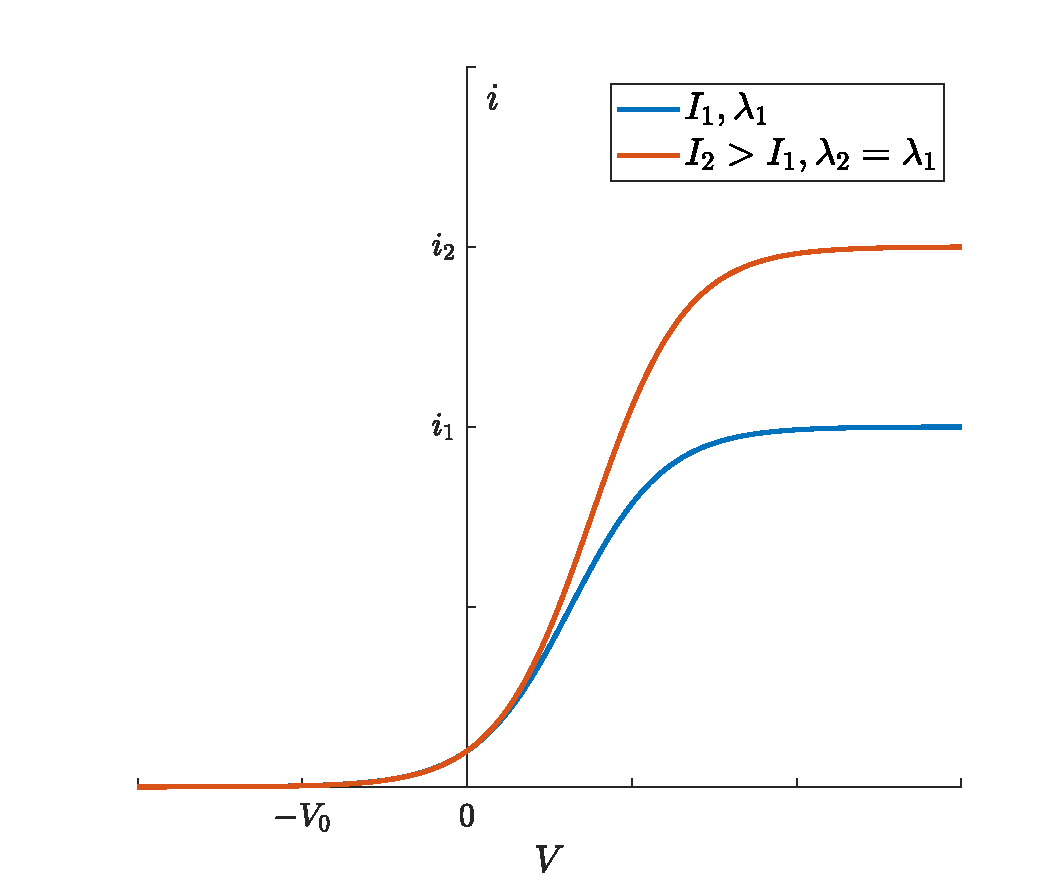
\includegraphics[width=\textwidth]{Seminar_02/pics/pic_01.pdf}
\column{0.45\textwidth}
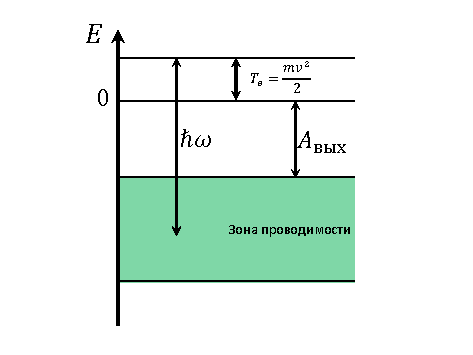
\includegraphics[width=\textwidth]{Seminar_02/pics/pic_02.pdf}
\end{columns}
\end{frame}

\begin{frame}[t]{Эффект Комптона}
\only<1>{
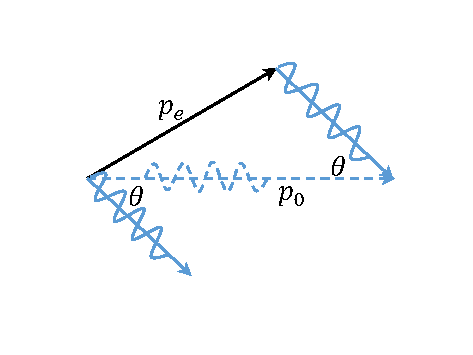
\includegraphics[width=\textwidth]{Seminar_02/pics/pic_03.pdf}
Дальнейший вывод в конспекте
}

\end{frame}







\begin{frame}{Задача 1.17}\scriptsize
\only<1>{
\begin{block}{Условие}
Какую минимальную длительность импульса фототока можно получить в вакуумном фотоэлементе, между анодом и катодом которого приложено напряжение в несколько сотен вольт, при освещении фотокатода короткими ($10^{-11}$ с) импульсами света с длиной волны $\lambda = 500$ нм. Красная граница материала фотокатода $\lambda_{\text{кр}} = 1000$ нм, напряженность поля между анодом и фотокатодом $E= 300$ В/см.
\end{block}
}
\only<2>{
\begin{block}{Решение}
Максимальная скорость выбиваемых электронов
\begin{gather*}
    \dfrac{mV_{max}^2}{2} = \hbar(\omega - \omega_0) = hc\left(\dfrac{1}{\lambda} - \dfrac{1}{\lambda_0} \right)\\
    V^2_{max} = \dfrac{2hc}{m}\left(\dfrac{1}{\lambda} - \dfrac{1}{\lambda_0} \right)
\end{gather*}
Кинематическая задачка о времени пролета электронов в трубке длиной $l$:
\begin{gather*}
    l = \dfrac{eEt_1^2}{2m} = V_{max}t_2 +\dfrac{eEt_2^2}{2m} \Rightarrow t_1 = t_2\sqrt{1+\dfrac{2mV_{max}}{eEt_2}}\\
    t_1 = t_2 + \dfrac{mV_{max}}{eE}
\end{gather*}
Здесь мы просто разложили этот корень с $t_2$, потому что значение добавки мало:
\begin{equation*}
    \Delta t = t_1 - t_2 = \dfrac{1}{eE}\sqrt{\dfrac{2hc}{m}\left(\dfrac{1}{\lambda} - \dfrac{1}{\lambda_0} \right)} = 1.2\cdot10^{-10} \text{с}
\end{equation*}
\end{block}
}
\end{frame}

\begin{frame}{Задача 1.32}\scriptsize
\only<1>{
\begin{block}{Условие}
 С какой скоростью $v$ должен двигаться электрон, чтобы летящий ему навстречу фотон с длиной волны $\lambda = 0,0024$ нм не изменил свою энергию при $180^\circ$-рассеянии?
\end{block}
}

\only<2>{
\begin{block}{Решение}
Закон сохранения энергии с учетом релятивистской энергии электрона, где $\beta = v/c$:
\begin{equation*}
    \hbar\omega + \dfrac{mc^2}{\sqrt{1+\beta^2}}=\hbar\omega + \dfrac{mc^2}{\sqrt{1+\beta^{'2}}}
\end{equation*}
Единственное решением это $\beta = \beta^'$, то есть электрон летит назад с той же скоростью назад.\\
Закон сохранение импульса:
\begin{gather*}
    \dfrac{\hbar\omega}{c} - \dfrac{mc\beta}{\sqrt{1+\beta^2}} = -\dfrac{\hbar\omega}{c} + \dfrac{mc\beta}{\sqrt{1+\beta^2}}\\
     \dfrac{mc\beta}{\sqrt{1+\beta^2}} = \dfrac{\hbar\omega}{c} = \dfrac{h}{\lambda}\\
     \dfrac{\beta}{\sqrt{1+\beta^2}} = \dfrac{h}{mc}\dfrac{1}{\lambda} = \dfrac{\lambdabar}{\lambda}\approx 1\\
\end{gather*}
Окончательно решаем уравнение на $\beta$ и находим, что $v = c/\sqrt{2}$
\end{block}
}
\end{frame}

\begin{frame}{Задача 1.48}\scriptsize
\only<1>{
\begin{block}{Условие}
Возбужденное ядро с энергией возбуждения $\Delta \epsilon = 1 $ МэВ с $A = 100$ движется с кинетической энергией $T = 100$ эВ и испускает $\gamma$-квант. Под каким углом к направлению движения ядра сдвиг $\gamma$-кванта по энергии будет равен нулю?
\end{block}
}
\only<2>{
\begin{block}{Решение}

Эффекта Допплера:
\begin{equation*}
    \omega = \omega_0 \left(1+ \dfrac{v}{c}\cos{\theta} \right)
\end{equation*}
При излучении гамма-кванта скорость у ядра тоже меняется\\
Импульсы ядра и гаммам-кванта в системе покоя ядра одинаковые и посчитаем это сдвиг частот:
\begin{gather*}
    \Delta\omega = \dfrac{T_{new}}{\hbar} =  \dfrac{p^2}{2m\hbar} = \dfrac{E^_{\gamma}}{2mc^2\hbar}\\
    \omega = \dfrac{E_{\gamma} - T_{new}}{\hbar} = \dfrac{E_{\gamma}}{\hbar}(1-\dfrac{E^_{\gamma}}{2mc^2})
\end{gather*}
С учетом этих двух сдвигов частот получаем:
\begin{equation*}
    \omega = \dfrac{E_{\gamma}}{\hbar} \left(1+ \dfrac{v}{c}\cos{\theta} - \dfrac{E^_{\gamma}}{2mc^2}\right)
\end{equation*}
И они должны скомпенсировать друг друга:
\begin{equation*}
    \dfrac{v}{c}\cos{\theta} = \dfrac{E^_{\gamma}}{2mc^2} \Rightarrow \cos{\theta} = \dfrac{E_\gamma}{v-2mc} = \dfrac{E_\gamma}{\sqrt{8Tmc^2}} \approx 0.116
\end{equation*}

\end{block}
}
\end{frame}



\begin{frame}[t]{Комментарии к задачам из задания}\scriptsize
\begin{itemize}
\item 0-2-1 Зная мощность светового потока можно спокойно найти импульс и удвоить его где нужно
\item 0-2-2 Подставить в формулу эффекта Комптона нужный угол
\item Задача 1.7 Нужно вспомнить разложение амплитудной модуляции в спектр и посмотреть кто выбивает электроны, а кто нет
\item Задача 1.18 Нужно как в первой неделе прикинуть сколько энергии приходит в атом и посчитать займет времени накопление энергии на фотоэффект
\item Задача 1.23 Нужно взять формулы из следствия уравнения Комптона
\item Задача 1.35 Решить задачу на эффект Комптона, только с движущимся электроном
\item Задача 1.39 Решена в задачнике
\item Задача 1.48 Решена 
\end{itemize}
\end{frame}

\end{document}